% calculus:x04 GDC:NO
\begin{question}
  \hspace*{\fill} [Note maximale: 15]\par
  \medskip
  \noindent La figure suivante donne la représentation graphique de $f(x) = a\,Cos\,bx $, pour $ 0 \le x \le 4$.\par  
  \medskip
  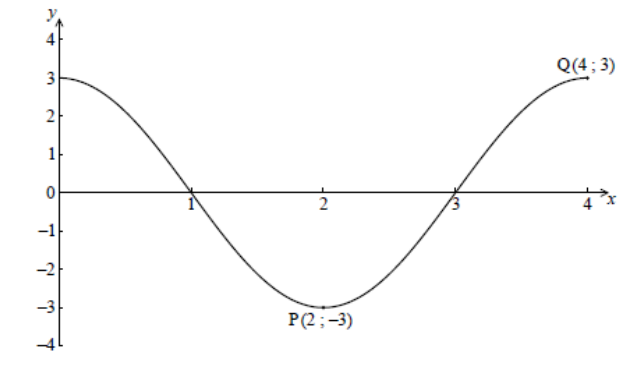
\includegraphics[scale=0.3]{temp_cos_wave}\par
  \medskip
  \noindent Il y a un point minimum en $P$ ( 2, -3 ) et un point maximum en $Q$ (4, 3).\par
  \medskip
  (a)\par
  \hspace{1em} (i)  Donnez la valeur de $a$.\par
  \medskip
  \hspace{1em} (ii) Trouvez la valeur de $b$.\hspace*{\fill} [3]\par
  \medskip
  (b) Donnez la pente de la courbe en P.\hspace*{\fill} [1]\par
  \medskip
  (c) Donnez l’équation de la normale à la courbe en P.\hspace*{\fill} [2]\par
  \medskip
\end{question}

